\chapter{El modelo central de la economía geográfica}

\section{Introducción}
\textbf{Como señalamos en el prefacio, hace mucho tiempo que Ohlin (1933) observó que los campos de la teoría del comercio por un lado y la economía regional y urbana por el otro tenían, en principio, los mismos objetivos de investigación. Ambas áreas de investigación quieren responder a las preguntas: ¿Quién produce qué, dónde y por qué?} A pesar de la observación de Ohlin, cada campo ha seguido su propio camino desde el siglo XIX. El capítulo 2 mostró que la teoría del comercio asume que los países son puntos adimensionales en el espacio. \textbf{Los teóricos del comercio están interesados principalmente en cómo interactúan la estructura del mercado, las técnicas de producción y el comportamiento del consumidor} (Neary, 2004). Los precios resultantes de los factores y las materias primas determinan el patrón de los flujos comerciales internacionales. La ubicación es, en el mejor de los casos, un factor exógeno y, por lo general, no juega un papel significativo. \textbf{La economía regional y urbana, por el contrario, toma la estructura del mercado y los precios como dados y trata de averiguar qué asignación de espacio es más eficiente}. El comportamiento subyacente de consumidores y productores, central en la teoría del comercio, es menos importante (Fujita y Thisse, 1996). Aunque ambas corrientes de la literatura producen ideas valiosas por derecho propio, \textbf{la teoría del comercio y la economía regional y urbana se combinan productivamente en la economía geográfica.}\\

Este capítulo analiza y explica el modelo central de la economía geográfica, un pequeño modelo de equilibrio general desarrollado por Krugman (1991a, 1991b). Como veremos, \textbf{las ecuaciones de equilibrio de este modelo no son lineales. Esto significa que los pequeños cambios en los parámetros no siempre producir los mismos efectos; a veces los efectos son pequeños, a veces son grandes.} Traducido a la economía regional y urbana, esto significa, por ejemplo, que la decisión de ubicación de un solo productor podría no cambiar el patrón espacial de producción, pero podría tener efectos dramáticos o catastróficos (tomando prestado un término de la literatura del caos). , Consecuencias. Es posible que la decisión de ubicación de un solo productor desencadene un proceso de causalidad acumulativa y que el patrón espacial de producción cambie drásticamente. Además, el modelo tiene múltiples equilibrios, y esta característica es, como hemos explicado en el capítulo 2, una de las principales diferencias con la ciencia regional o la economía urbana. No se presupone qué la ubicación podría convertirse en el centro de producción, pero una vez que una ubicación obtiene una ventaja, el proceso de causalidad acumulativa comienza a funcionar. Lo que inicialmente son pequeñas diferencias entre ubicaciones pueden evolucionar con el tiempo en grandes diferencias en el equilibrio a largo plazo. Estas y otras características hacen que los modelos de economía geográfica sean analíticamente complicados.\\

\section{Un ejemplo de la economía geográfica}
Es posible construir un ejemplo simple para ilustrar algunos de los principales hallazgos del enfoque de economía geográfica. Supongamos que hay dos regiones (o países), Norte y Sur, y dos sectores de producción, manufactura y agricultura. La industria manufacturera produce variedades, es decir, productos diferenciados, bajo economías internas de escala. Por lo tanto, el costo por unidad de producción cae a medida que una empresa expande su nivel de producción. Como resultado, cada empresa produce solo una variedad. Una empresa puede residir en el Norte o en el Sur, es decir, una empresa tiene que decidir dónde producir. Esta decisión de ubicación diferencia esencialmente el ejemplo de la nueva teoría comercial.\\
\begin{center}
\begin{tabular}{lccc}
    &Ventas norte&Ventas sur& Ventas totales\\\\
    \hline\\
    Todas las empresas en el norte & 5+5=8 & 0+2=2 & 10\\
    Todas las empresas en el sur & 0+4=4 & 4+2=6 & 10\\
    $25\%$ de empresas en el norte, & 1+4=5 & 3+2=5 & 10\\
    $75\%$ de empresas en el sur. & & & \\\\
\end{tabular}
\end{center}

La demanda total de cada variedad de manufacturas en este ejemplo es exógena. Suponemos que cada empresa vende cuatro unidades a los trabajadores de la industria manufacturera y seis unidades a los agricultores. Por lo tanto, la demanda total de cada variedad es diez (6 + 4). La producción de la agricultura, y por lo tanto la demanda que genera, es específica de la ubicación. Su distribución espacial está dada exógenamente; suponemos que se venden cuatro unidades en el Norte y dos unidades en el Sur. La ubicación de los trabajadores en el sector manufacturero y, por tanto, las cuatro unidades que demandan en esa ubicación, no es exógena. El papel de los trabajadores inmóviles es importante, ya que aseguran que siempre haya una demanda positiva en ambas regiones. Finalmente, los costos de transporte entre el Norte y el Sur son 1 euro por unidad. Las empresas deciden su ubicación para minimizar los costos de transporte.\\
Ahora podemos determinar la decisión de ubicación de cada empresa. Primero, podemos calcular las ventas regionales de cada empresa, dada la ubicación de las otras empresas. En la tabla de arriba, se dan tres posibilidades (no exhaustivas): todas las empresas en el Norte, todas las empresas en el Sur y el 25 por ciento de todas las empresas en el Norte y el 75 por ciento de todas las empresas en el Sur. Las ventas en cada región son iguales a las ventas a los trabajadores en la manufactura más las ventas a los agricultores. Tomemos, por ejemplo, la última fila de la tabla.  La empresa vende cinco unidades en el Norte, a saber, cuatro a los agricultores ubicados en Norte más un ($ = 25\% · 4)$ unidad a los trabajadores de manufactura ubicados en Norte. De manera similar, la empresa vende cinco unidades en el Sur, es decir, dos unidades a los agricultores ubicados en el Sur más tres $( = 75\% · 4)$ unidades a los trabajadores de manufactura ubicados en el Sur.\\
En segundo lugar, usando la tabla podemos construir una tabla de decisión, calculando los costos de transporte en función de la decisión de ubicación de la empresa, dada la ubicación de las otras empresas. Suponga, por ejemplo, que todas las empresas están ubicadas en el norte. La tabla de abajo indica que los costos de transporte para una empresa ubicada en el Sur serán entonces 8 euros, es decir, 4 euros para las ventas a los agricultores del Norte y 4 euros para las ventas a todos los trabajadores de la industria manufacturera ubicada en el Norte (haciendo abstracción de las ventas a sus propios trabajadores). De manera similar, si la empresa se ubica en el norte, los costos de transporte serían solo 2 euros para las ventas a los agricultores del sur. Dado que los costos de transporte se minimizan al ubicarse en el Norte si todas las demás empresas están ubicadas en el Norte, la empresa decide ubicar también la producción en el Norte. Como muestra el cuadro  (segunda fila), una empresa se ubicará en el Sur si todas las demás empresas también se ubican allí, mientras que (última fila) a la empresa le es indiferente ubicarse en el Norte o en el Sur (ya que los costos de transporte son los mismos si la empresa se ubica en el Sur). En cualquier región si el 25 por ciento de las empresas están ubicadas en el Norte y el 75 por ciento en el Sur.

\begin{center}
    \begin{tabular}{lcc}
	& Ubicado en el Norte & Ubicado en el sur \\\\
	\hline\\
	Todas las empresas Norte & 0+\textbf{2}=2 (Agricultores Sur) & 4+4=8 (Trabajadores y agricultores Norte)\\
	Todas las empresas Sur &4+2=6 (Trabajadores y agricultores Sur)& 0+4=\textbf{4} (Agricultores Norte)\\
	$25\%$ de agricultores Norte, & 3+2=5 (trabajadores y agricultores Sur) & 1+4=5 (Trabajadores y agricultores Norte)\\
	$75\%$ de agricultores Sur & &  \\
	\hline\\
    \end{tabular}
    Costos de transporte
\end{center}
\vspace{.5cm}

En primer lugar, el concepto de causalidad acumulativa. Si, por alguna razón, una ubicación ha atraído a más empresas que la otra ubicación, una nueva empresa tiene un incentivo para ubicarse donde están las otras empresas. Tome la primera fila en la tabla de arriba. Si todas las empresas existentes están ubicadas en el norte, la nueva empresa también debería ubicarse allí si desea minimizar sus costos de transporte. De manera similar, para la segunda fila,  la empresa se ubicará en el sur.\\
En segundo lugar, la tabla  ilustra la existencia de equilibrios múltiples. La aglomeración de todas las empresas en el Norte o en el Sur es un equilibrio. Sin embargo, no podemos determinar de antemano dónde ocurrirá la aglomeración. Esto depende críticamente de las condiciones iniciales, es decir, las decisiones previas de ubicación de otras empresas.\\
Tercero, un equilibrio puede ser estable o inestable. Las entradas en negrita en la tabla  son ambos equilibrios estables si una sola empresa decide mudarse, esto decisión no influiría en las decisiones de ubicación de las otras empresas. La última fila  describe un equilibrio inestable. Si una sola empresa decide trasladarse, la nueva ubicación se volverá inmediatamente más atractiva para todas las demás empresas. Esto desencadenará un efecto bola de nieve: todas las empresas seguirán al pionero. En este ejemplo, solo la aglomeración es un equilibrio estable.\\
En cuarto lugar, observamos que un equilibrio estable puede no ser óptimo. Si todas las empresas están ubicadas en el norte, los costos de transporte son solo 2 euros. Si todas las empresas están ubicadas en el sur, los costos de transporte son 4 euros.  Por lo tanto, los costos de transporte para la economía en su conjunto se minimizan si todas las empresas se aglomeran en el Norte, mientras que la aglomeración en el Sur sigue siendo un equilibrio estable.\\
En quinto lugar, el ejemplo ilustra la interacción de la aglomeración y los flujos comerciales. Con la aglomeración completa, es decir, todas las manufacturas se producen en una sola región, el comercio entre regiones será de tipo interindustrial (alimentos para manufacturas). De hecho, este equilibrio también refleja el llamado efecto del mercado doméstico; la combinación de economías de escala y costos de transporte es responsable del agrupamiento de toda la actividad libre en un solo lugar. Debido a esta combinación, los costos de transporte pueden minimizarse. La gran región termina con un gran mercado para la fabricación de bienes, que pueden venderse sin incurrir en costos de transporte. La consecuencia es que esta región se convierte en exportadora de productos manufacturados; Las grandes regiones tienden a convertirse en exportadoras de aquellos bienes para los que tienen un gran mercado local, de ahí el término efecto del mercado interno. Si la industria manufacturera está ubicada en ambas regiones, como se describe en las últimas filas de los cuadros, el comercio también será del tipo intraindustrial. Además de intercambiar bienes manufacturados por productos agrícolas, se intercambiarán diferentes variedades de productos manufacturados diferenciados entre ambas regiones.\\
El ejemplo es útil, ya que ilustra algunos aspectos importantes de la economía geográfica. Sin embargo, un ejemplo es solo un ejemplo y no es un sustituto de un modelo bien especificado. ¿Qué falta en el ejemplo?\\
\begin{itemize}
    \item \textbf{En primer lugar, falta la interacción entre los costos de transporte, el comportamiento de fijación de precios y la elección de la ubicación.} Simplemente suponemos que la demanda que enfrenta cada empresa está dada y es independiente del comportamiento de fijación de precios y los costos de transporte. De hecho, los precios faltan por completo en el ejemplo. No hay análisis de la estructura del mercado. En realidad, los precios, los salarios y los costos de transporte determinarán el poder adquisitivo de los consumidores. Uno podría suponer que esta interacción impulsa las decisiones de ubicación de consumidores y productores. Las siguientes secciones muestran que este es, de hecho, el caso.
    \item Además, es un modelo de equilibrio parcial, en el sentido de que las empresas no se preocupan por la mano de obra necesaria; donde sea que decidan ubicarse, \textbf{la disponibilidad de mano de obra no es el problema.} Resultará que los supuestos con respecto al funcionamiento del mercado laboral son importantes. El lector también puede notar la similitud del ejemplo y el nuevo modelo de comercio de Krugman (1980) discutido en el capítulo 2. En ambos modelos, las economías de escala y los costos de transporte son fuerzas importantes. La diferencia más importante es que, en nuestro ejemplo, las empresas pueden ubicarse en cualquier región. En consecuencia, el ejemplo da lugar a aglomeraciones y equilibrios múltiples.
\end{itemize}

\section{La estructura del modelo.}

Esta sección ofrece una descripción general no técnica de la estructura general del modelo central de la economía geográfica. Los aspectos básicos del modelo central se exponen en Dixit y Stiglitz (1977) y Krugman (1979, 1980). Estos trabajos estimularon una gran cantidad de trabajo sobre competencia monopolística y teoría del comercio internacional. Krugman (1991a, 1991b) extiende este último al permitir la movilidad de factores interregionales, y esto se ha convertido en el modelo central de la economía geográfica. Esta estructura se ilustra en la figura de abajo. \\
El modelo central identifica dos regiones, etiquetadas como 1 y 2. Hay dos sectores en la economía, el sector manufacturero y el sector alimentario. Los consumidores en ambas regiones consisten en trabajadores agrícolas y trabajadores de manufactura. Los trabajadores agrícolas obtienen sus ingresos trabajando en las granjas de su región. El flujo de ingresos de los trabajadores agrícolas es parte de una transferencia bilateral: obtienen un ingreso a cambio de su oferta de mano de obra. Todas esas transferencias bilaterales se indican con flechas de dos puntas. La flecha de punta sólida indica la dirección de los flujos de dinero o ingresos, es decir, indica la dirección de los ingresos y los gastos. Lo que representa el flujo se indica a lo largo de la línea que conecta los puntos de flecha. La flecha de punta abierta indica la dirección de los flujos de bienes o servicios. Estos se indican entre paréntesis a lo largo de la línea que conecta los puntos de flecha. \textbf{Los agricultores de la región 1 producen alimentos bajo rendimientos constantes a escala y competencia perfecta}. Venden este alimento a los consumidores, ya sea en la región 1 o en la región 2. Por supuesto, no hay costos de transporte para los alimentos.\\

\begin{center}
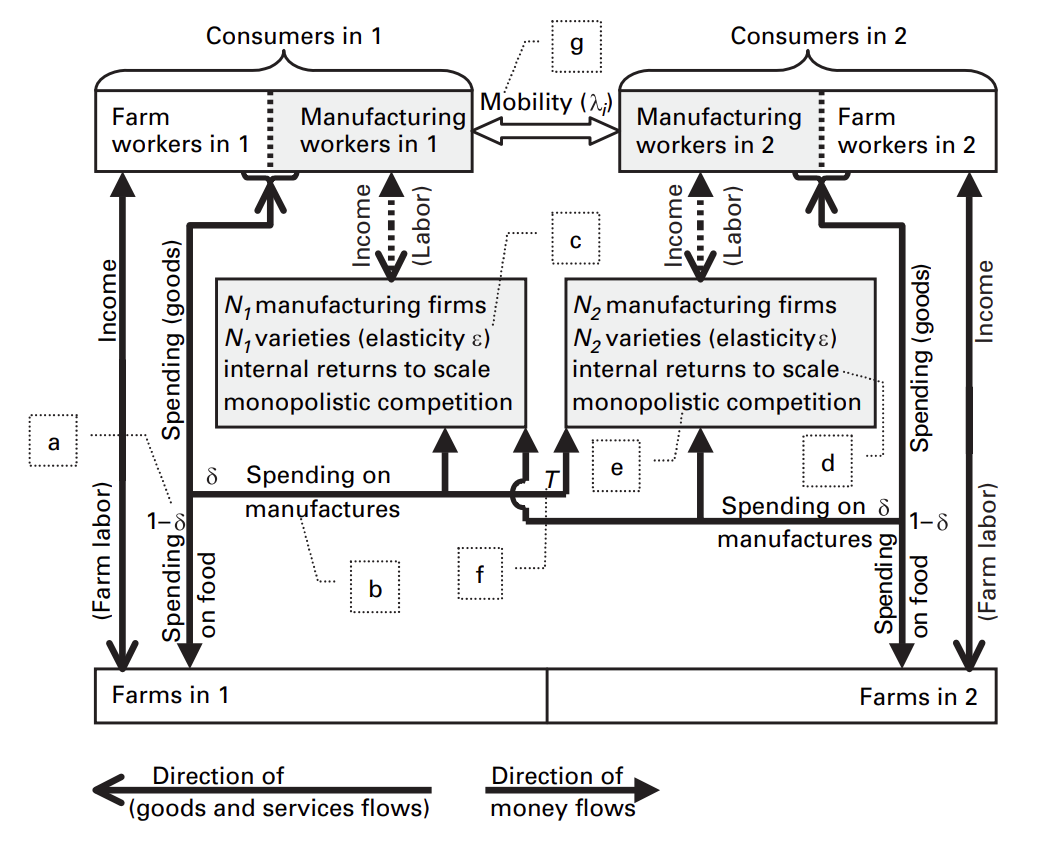
\includegraphics[scale=.4]{./imagen/diag.png}
\end{center}

El sector manufacturero consta de empresas $N1$ en la región 1 y empresas $N2$ en la región 2. Cada empresa manufacturera produce un producto diferenciado, es decir, produce una variedad única de manufacturas. \textbf{Utiliza solo mano de obra en el proceso de producción, que se caracteriza por economías internas de escala. Esto implica que las empresas tienen poder de monopolio, que utilizan para determinar el precio de su producto. Además, los costos de transporte están involucrados en la venta de un bien manufacturado en otra región. Estos costos no surgen si el bien manufacturado se vende en la región en la que se produce. Como resultado de los costos de transporte, las empresas exportadoras cobrarán un precio más alto en la región extranjera que en la región de origen.} Los trabajadores manufactureros obtienen sus ingresos (la tasa salarial manufacturera) al suministrar mano de obra a las empresas del sector manufacturero ubicadas en la región de origen.\\
Los consumidores gastan sus ingresos tanto en alimentos como en manufacturas. Dado que los alimentos son un bien homogéneo, no les importa si se producen en la región 1 o en la región 2. Como los alimentos no tienen costos de transporte, tienen el mismo precio en ambas regiones (lo que implica que los agricultores ganan el mismo salario en ambas regiones). El gasto de los consumidores en manufacturas debe distribuirse entre las muchas variedades producidas en las regiones 1 y 2. \textbf{En igualdad de condiciones, consumir variedades importadas es más costoso que consumir variedades nacionales, como resultado de los costos de transporte de los productos manufacturados.} Sin embargo, dado que las variedades son productos diferenciados y los consumidores tienen gusto por la variedad, siempre consumirán algunas unidades de todas las variedades producidas, ya sea en el país o en el extranjero.\\
Se imponen algunas observaciones finales sobre la figura. Primero, la figura menciona los parámetros más importantes que se usarán en el resto de este libro, a saber, $\epsilon, \delta, \lambda_i$ y $T$. En este punto no es importante saber cuáles son estos parámetros. Ellos, y otros, serán discutidos en el resto de este capítulo. En segundo lugar, la figura  muestra siete rótulos, etiquetados de la $a$ la $g$. Estas anotaciones se refieren a detalles de construcción importantes del modelo central. Se utilizan como referencia y recordatorio en la sección 3.4 sobre la estructura de demanda del modelo (rótulos a, b y c), en la sección 3.5 sobre la estructura de oferta del modelo (rótulos d y e), en la sección 3.6 sobre el papel de los costos de transporte (llamada f) y en la sección 3.9 sobre la dinámica del modelo (llamada g). En tercer lugar, y lo más importante, hay cuadros sombreados en la figura. Estos llaman la atención sobre la característica distintiva de la economía geográfica: la movilidad de los factores de producción. El modelo central aplica la movilidad solo al sector manufacturero; los trabajadores de fabricación pueden trasladarse de la región 1 a la región 2, o viceversa. \textbf{La reubicación de empresas manufactureras de una región a otra es la otra cara de la misma moneda, ya que una expansión de la mano de obra manufacturera en una región implica una expansión de la producción en el sector manufacturero.} Es importante señalar que, en principio, las casillas sombreadas pueden desaparecer en una región, por ejemplo, si todos los trabajadores de fabricación (y, por lo tanto, todo el sector manufacturero) se trasladan a la región 2. Las casillas no sombreadas, etiquetadas como trabajadores agrícolas y granjas, no pueden desaparecer de una región. Los agricultores necesitan la tierra para el cultivo y, por lo tanto, no son móviles. La región, por lo tanto, siempre puede gastar los ingresos generados por este sector. La distinción entre actividad móvil y actividad inmóvil es importante. Para facilitar la referencia, hemos etiquetado estos sectores como manufacturas y alimentos, respectivamente. Obviamente, el sector inmobiliario también podría producir mineral de hierro o papel, o producir un servicio no transable (vivienda), etc.\\

\paragraph{Terminología}

\textbf{Aglomeración y dispersión.} Estamos interesados en explicar y describir varias formas de agrupación de actividad (económica), a las que nos referimos como aglomeración. Usamos el término difusión para referirnos a lo contrario de aglomeración. Otros términos utilizados en la literatura, como centrípeto, centrífugo, convergente y divergente, no se utilizarán en este libro porque pueden ser confusos. Por ejemplo, la palabra convergente puede indicar que todas las industrias convergen, es decir, tienden a ubicarse en una región, o que todas las regiones convergen, es decir, todas las industrias están distribuidas entre regiones.\\
\textbf{Numerario}. Los agentes económicos en los modelos de equilibrio general de la economía geográfica no sufren de ilusión monetaria, es decir, sus decisiones se basan en precios relativos y no dependen del nivel absoluto de precios. Esto nos permite establecer el precio de uno de los bienes del modelo igual a uno, y expresar todos los demás precios del modelo en relación con el precio del bien numerario. El resto del libro elige la comida como bien numerario, de modo que el precio de la comida siempre es igual a uno.\\
\textbf{Salarios y salarios reales.} El enfoque central de modelado de equilibrio general utilizado en este libro elige un bien numérico para precisar los precios relativos. Los salarios en diferentes regiones expresados en el numerario deben denominarse salarios numerarios. Aunque es mejor que el término de uso frecuente salarios nominales (ya que el sector monetario no se modela explícitamente), sigue siendo un término engorroso. Por lo tanto, usamos el término más corto salario cada vez que nos referimos a salario numérico, y usamos explícitamente el término salario real cuando los salarios numéricos se corrigen por el nivel de precios para determinar el poder adquisitivo.

\section{Demanda}



